\begin{boxC}
    نتایج مربوط به آزمایش ما برای مدل‌کردن 
    \lr{Topic}
    ها به شرح زیر است.
    به ازای هر کدام از تعداد 
    \lr{Topic}
    بین ۳ تا ۱۵ 
    امتیاز
    \lr{Coherent Score}
    به شرح زیر است : 
\end{boxC}

\begin{figure}[h]
    \centering
    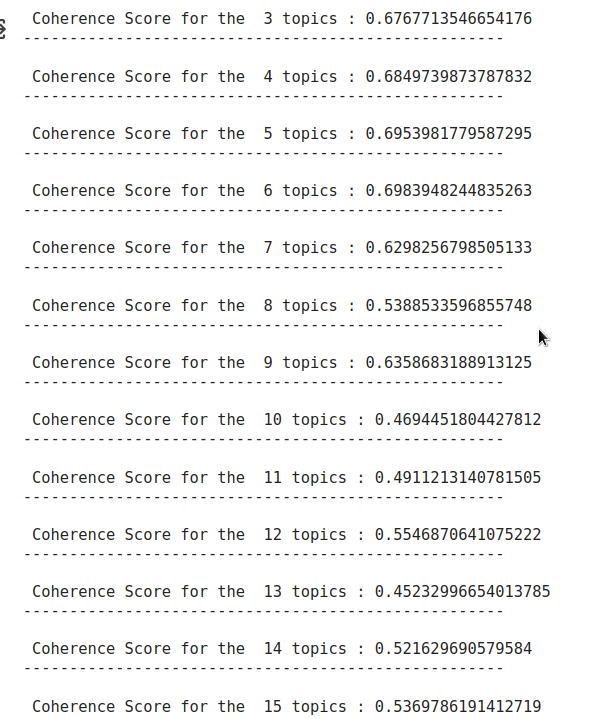
\includegraphics
    [width = 0.8\textwidth]
    {IR6/images/LDA.png}
    \caption{\lr{Coherence Scores for topic modeling}}
    \label{fig:enter-label}
\end{figure}

\begin{boxL}
    همانطور که از تصویر بالا مشخص است ، بهترین امتیاز مربوط به تعداد ۵ یا ۶ 
    \lr{Topic}
    می‌باشد . 

    امتیاز انسجام معیاری برای سنجش کیفیت موضوعات تولید شده توسط الگوریتم LDA (تخصیص دیریکله نهفته) در مدل سازی موضوع است. درجه تشابه معنایی بین کلمات با امتیاز بالا در یک موضوع را اندازه گیری می کند. به عبارت دیگر، میزان معناداری و تفسیرپذیر بودن موضوعات را می سنجد.

امتیاز انسجام بر اساس N کلمه برتر در هر مبحث و همزمانی این کلمات در پیکره مرجع محاسبه می شود. مجموعه مرجع مجموعه بزرگی از اسناد است که به حوزه مورد علاقه مرتبط هستند. امتیاز انسجام بین 0 تا 1 است که نمرات بالاتر نشان دهنده موضوعات منسجم تر و قابل تفسیرتر است.

\textbf{
به نظر می‌رسد که یک میزانی از حد برای تعداد مناسب 
\lr{Topic}
برای هر مجموعه
\lr{DataSet}
وجود دارد.
در این مجموعه داده ما این تعداد برابر ۵ و ۶ می‌باشد.
}
\end{boxL}

\begin{figure}[h]
    \centering
    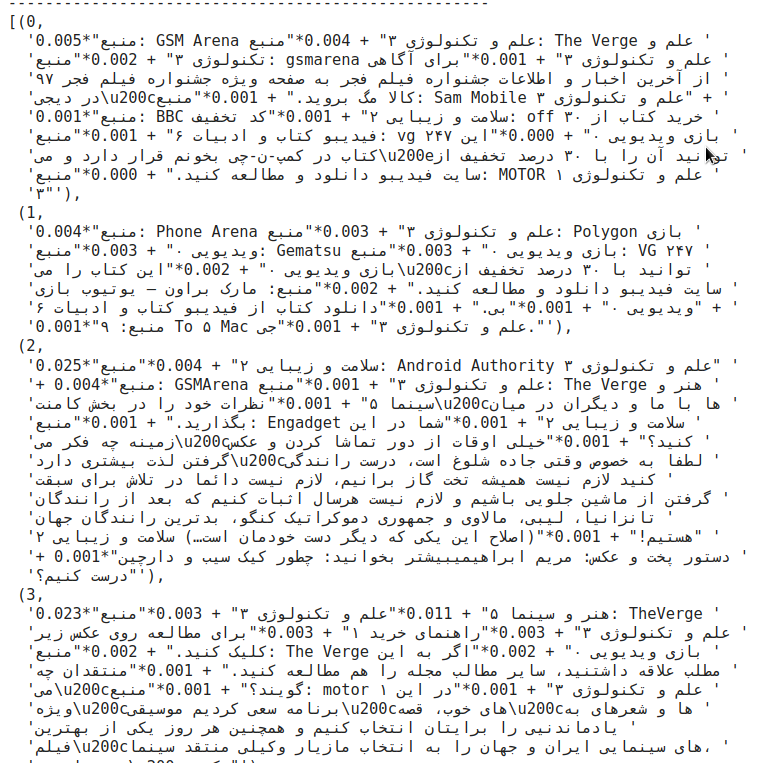
\includegraphics
    [width = 0.8\textwidth]
    {IR6/images/LDA_a.png}
    \caption{\lr{Topics for 6 topics (1)}}
    \label{fig:enter-label}
\end{figure}


\begin{figure}[h]
    \centering
    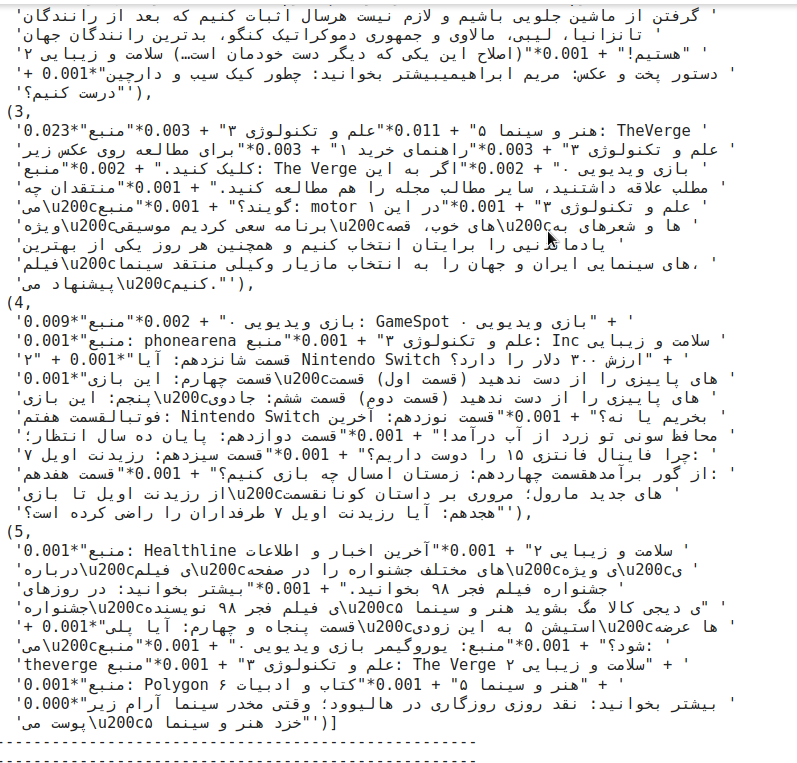
\includegraphics
    [width = 0.8\textwidth]
    {IR6/images/LDA_b.png}
    \caption{\lr{Topics for 6 topics (2)}}
    \label{fig:enter-label}
\end{figure}